%FREELY FALLING BODY
\newexp

\section*{Before Lab}

Please read this writeup carefully. At many points the writeup asks
questions and reports things
you should address in your notebook (e.g., ``Explain why in your notebook").
A good strategy is to highlight or underline each question mark and ``explain why"
as you read so you can quickly
find them and confirm that you have answered each of them before you turn in your notebook.
Please also continue reading
in the Appendices to this manual.  This experiment particularly stresses
material from Appendices A and D.

\section*{Introduction}
     Two objects with the same size and shape but different mass are
     shown to you.  Then someone asks:
Which will fall faster, the heavy one or the light one?
Aristotle (about 300 B.C.)  gave his philosophical arguments
which concluded that the heavy one fell faster.  This misleading
 impression was challenged by
Galileo in about 1600.

As part of his analysis, Galileo investigated the properties of bodies
moving with constant acceleration, a subject that is still central to
our ideas of motion. In this experiment we will study free fall experimentally
and compare our result with theoretical equations of motion---are our
experimental results consistent with a constant acceleration?  And if so,
what is that acceleration.

  Another important goal of this experiment is to develop your
ability to analyze data scientifically.

\section*{Analysis of the Problem}
Two equations of motion that describe free fall with constant
acceleration are
\begin{equation}
v(t) = v_{\circ} + gt  \label{eq:v(t)}
\end{equation}
 and
\begin{equation}
x(t) = x_{\circ} + v_{\circ}t + {{1} \over {2}} gt^{2}  \label{eq:x(t)}
\end{equation}
where $x$ and $v$ represent position and velocity, $t$ the time, $x_{\circ}$ and
$v_{\circ}$ the position and velocity at $t = 0$, and $g$ is the acceleration
of gravity.  Your textbook should have a discussion of these equations,
which assume constant gravitational
acceleration, $g$, and negligible air resistance.  To study free fall in
our experiment, we will want to measure both the distance fallen, and velocity,
 as functions
of time.  Analysis of these
data (see pages~\pageref{scierror}--\pageref{compassis}) would give us the
functional relationships
between $v$,$t$ and $x$,$t$.  If the experimental relationships agree
with Eqs.~\ref{eq:v(t)}~and~\ref{eq:x(t)} above then the parameters determined
experimentally can be used to arrive at a value for $g$.

%     If we solve Eq.~\ref{eq:v(t)} for $t$ and substitute in Eq.~\ref{eq:x(t)},
% after a
%little algebra we obtain
%\begin{equation}
%v^{2} = v_{\circ}^{2} + 2g(x - x_{\circ})
%\end{equation}
%where $v$ is the velocity after the object has fallen a distance $x$
%and $v_{\circ}$ is the initial velocity.  To test this result
%experimentally we must have measured values of $x$ and $v$.

\section*{Experimental Methods}
     The apparatus is a Behr free fall apparatus shown
schematically in Fig.~\ref{fig:behr}.  {\bf CAUTION:} {\em This apparatus
produces very high voltages at very low currents.  It is unlikely to
be dangerous, but it is possible to get a painful shock.}
\begin{figure}
\begin{center}
{\resizebox{5in}{!}{{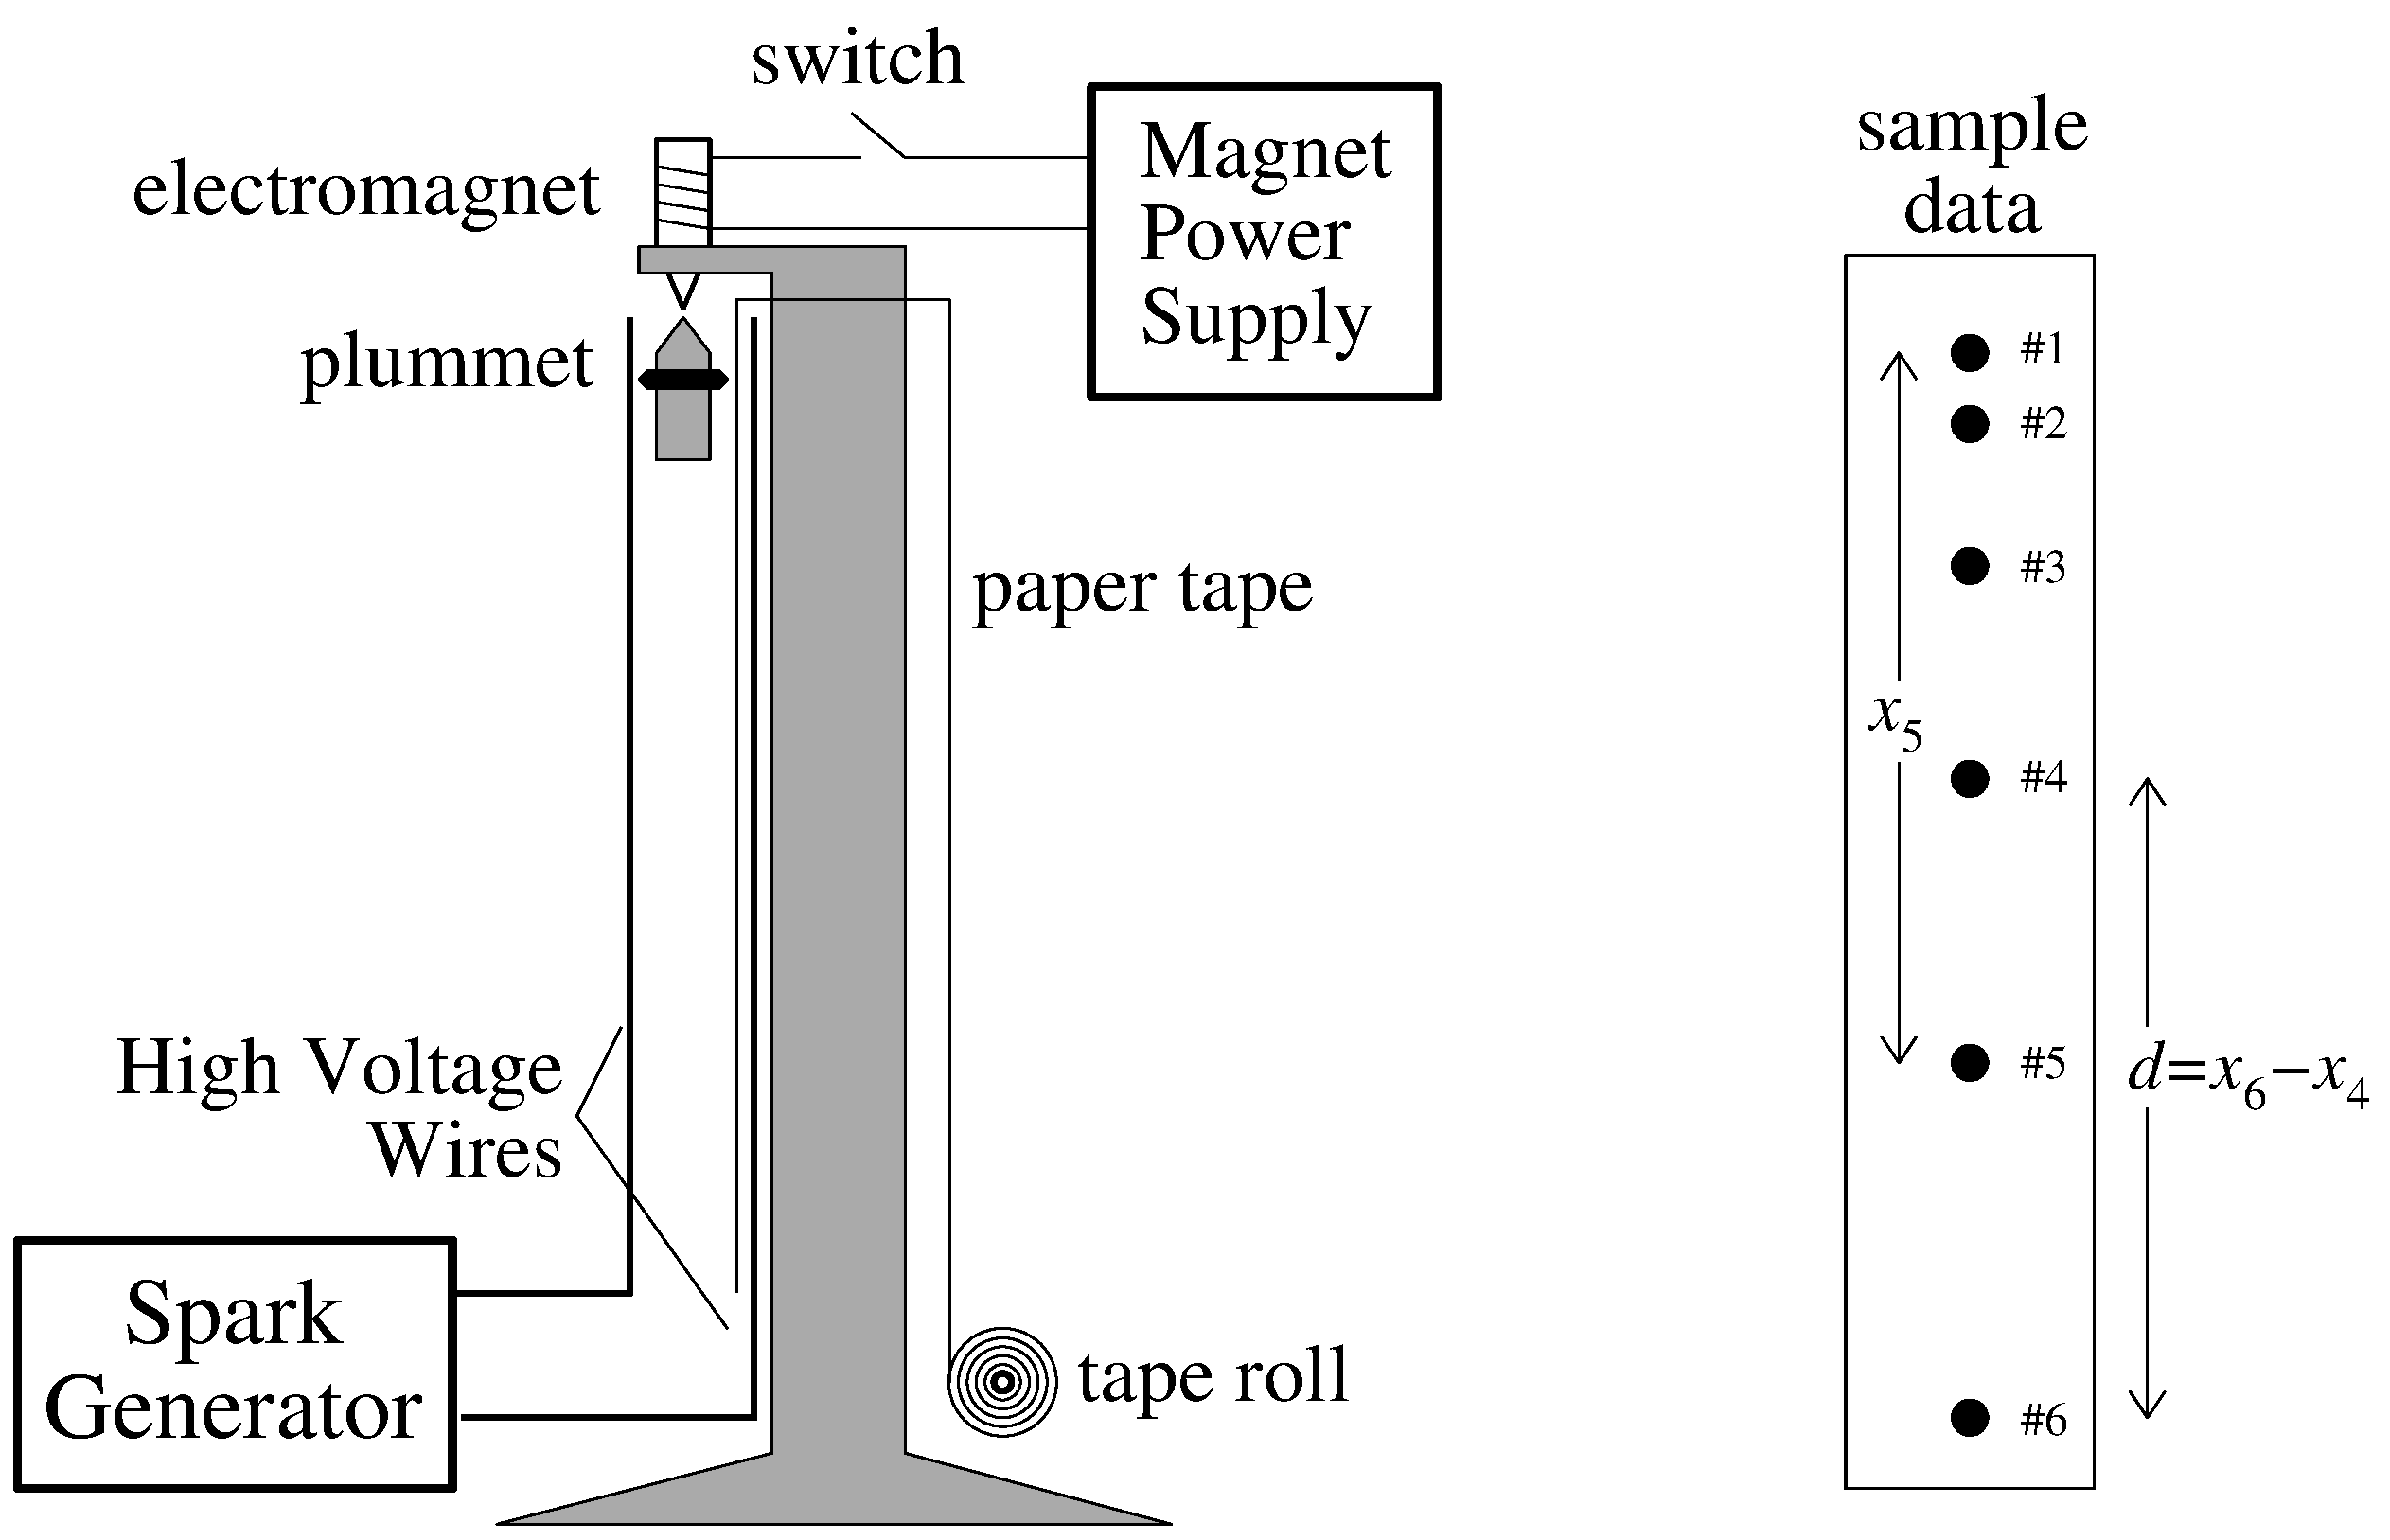
\includegraphics{behr2C.eps}}}}
\end{center}
%   \centerbmp{5in}{3.1in}{behr2.bmp}
 \caption{Behr Free Fall apparatus with sample data.  \label{fig:behr}}
\end{figure}
Check everything out with the instructor before using it.  When the switch to
the electromagnet is opened the plummet will fall freely.  The sparking system
will produce a spark hole through the sensitive paper every 1/60 of a second.
Since the spark jumps from the plummet to a wire behind the paper each spark hole marks
the position of the plummet at each spark time.  The resulting paper tape is thus a
record of distance fallen versus time.

%write and insert Appendix discussing Mean Speed Theorem
What about velocity as a function of time?  The instantaneous velocity is not
directly recorded on the paper tape.  Fig.~\ref{fig:behr} also shows a typical
section of tape with the dots representing spark holes at equal time intervals.
Using the Mean Speed Theorem, it can be shown that when the
acceleration is constant the instantaneous velocity at time $t_{5}$ is
numerically equal to the average velocity over the time interval $t_{4}$ to
$t_{6}$.  Hence from the information on the tape the velocity at time $t_{5}$
can be calculated by
\[
v(t_{5}) = {{d} \over {t_{6} - t_{4}}} = {x_6-x_4 \over t_{6} - t_{4}}
\]
We can use this trick for any combination of three successive dots on the tape
and thus determine the velocity as a function of time.

{\bf NOTE:} The choice of appropriate units for time can save you
a great deal of tedious computation. You will measure time
in units 1/60 sec, which we call a {\em wink} and velocity
 in units of cm per wink. Accelerations will come out in
cm/${\rm wink}^2$. After
you have completed the graphical and computer analysis and found
values for $g$, you can do a single unit conversion to
convert time back to seconds.  Ask your instructor or your TA if you
are not clear how to proceed.

\section*{Basic Procedure}
\begin{enumerate}\setcounter{enumi}{-1}
\item Read through {\em all} of this basic procedure and the following sections
on Uncertainties and Spreadsheet before beginning any measurements.

\item Ask the instructor to explain the operation of the apparatus to you.  Be
sure the apparatus is level, so the plummet will drop into the cup, and not hit
the wires on the way down.  Also, be sure you know how to operate the sparking
system without shocking yourself!

%If you think the apparatus is not level, ask {\em your TA} to level it
%for you.

\item Before installing the sensitive paper tape, make one or two trial runs
(Does the plummet drop without hitting wires?  Can you see sparks all the
way down the wires?  Don't touch the apparatus while the spark is on.)

\item Install the paper tape and take a final run to obtain data.

\item Remove the paper tape and check it immediately to see if all spark holes
are present (rerun if necessary).

\item Circle the spark holes and number them for convenience in making
measurements.

\item Decide what measurements you will make (see following on Uncertainties) and plan a data table 
accordingly.

\item Measure distances in cm.
Also, estimate the uncertainty in your
measurements of distance. (This uncertainty, $\delta x$, is probably the
same for every data point.)  Record the times, distances, and
uncertainties in the distances in a neatly constructed table.
%
\item Using your data, calculate velocity as a function
of time and enter the values
into your data table.  {\bf Note:}  You can calculate
the velocities with a calculator, but many people find it easier to use a
spreadsheet program---see below for detailed instructions.  
Also calculate the error in velocity.

\item  Analyze the $v(t)$ vs.\ $t$ data.  (A linear relationship is expected.)
Note: jumps in the $v(t)$ vs.\ $t$ graph usually indicate a missed spark hole.

\item Analyze the $x(t)$ vs.\ $t$ data.  (A quadratic relationship is expected.)

%\item Use the graph of $v(t)$ vs.\ $t$ to make a preliminary test of
%experimental validity---that is, see if all of your points appear to
%lie on a straight line.  It is easy to make an error in the
%calculations, but such errors will usually stand out prominently on
%a graph.  You are welcome to use Linfit to make the graph for this
%step.

%\item Do as much more of the data reduction and analysis as you have time
%for---it can be a help to do some of this work while help is available if
%needed.  Have the TA
%approve and initial your data before you leave.
\end{enumerate}

\section*{Uncertainties}

The uncertainties in this lab depends on the method
you use to reduce and analyze the data.  Two possibilities are listed below:
\begin{itemize}
\item[a.]  With the meter stick held firmly in place and {\em not}
zeroed on any particular spark hole, measure
the location $x$ of each spark hole.  Record the uncertainty  $\delta x$ of that
measurement. Note
that you will {\em not} want to use the first few marks on the
tape---they are usually  poorly defined.

Then, to find the velocities in units of
$\rm{cm}/{\rm wink}$, \underline{calculate}
the distances between every other point
using the individual $x$ values (e.g., $d_{4} = x_{5} - x_{3}$)
and then divide by 2 winks. (Why?)
%        If you use these units initially, you do not need to divide by
%        the time difference---see the explanatory note above.
	
In this case each individual value for $d$ has an uncertainty of
$\delta d = \sqrt{2} \cdot \delta x$.  Do you see why?  (Explain
this point in your writeup. Hint: see Eq.~E.5.) Divide $\delta d$ by 2 to get the uncertainty
in $v$. (Explain this point in your writeup. Hint: see Eq.~E.2.)

%{\em This method is strongly preferred.}

\item[b.]  Find the velocity directly by \underline{measuring}
the distance between every other point in addition to measuring
the location of each spark hole.
This method would give velocities with a bit better accuracy than the
first method, but would take twice as much time.
%give much less accurate results for the
%distance as a function of time, particularly for the data points
%towards the end of the tape.

%The reason is as follows: For each point, the distance from some
%starting
%point $x_0$ would have to be calculated from the measured $d$ values.
%Each of those values would have an error, so that the more values
%being added to find a given $x_i$, the larger the uncertainty for that
%point.  It is surprising but true that the method of reducing the data
%can affect the accuracy of the experiment!!

% 	\item[c.]  Measure the distance between each adjacent
% pair of points, picking
% up the meter stick each time and aligning it on the first point.  This
% method might seem reasonable, but in fact leads to much larger
% experimental errors.
%
%Let's call these measurements you made between points $p \pm \delta
%p$.  If you find a total distance $x$ travelled from the starting
%point, then each distance you measured must be added to the last
%total.  For example, the distance to the fourth point would be $x_4
%~=~
%p_1 + p_2 + p_3 + p_4$. That
%means that for each value of $x$ that you report,  the uncertainty
%will increase by $\delta p$.  Using the same example, $\delta x_4 ~=
%\delta p_1 + \delta p_2 + \delta p_3 + \delta p_4$.  As you can see, the
%uncertainty in the distance $x$ would be very large by the end of
%the tape!

\end{itemize}
Using either method will probably result in the same uncertainty
for every data point.  As a result \WAPP can calculate your
errors using a ``formula" (really just a constant), rather than using
individually determined errors for each datum.

%In each case you might choose a different value of raw data error.  In
%case a.  you probably listed a value for $\delta x$ of   %roughly $\pm~$0.5 mm.
%a few tenths of a millimeter.  In cases b.  and c.  you must deal with
%uncertainty
%at {\em both} ends of the meter stick, which should result in a larger
%uncertainty value.  It's your decision, so estimate the value that you
%think is prudent, and then later on you can check the accuracy of your
%estimate by scrutinizing the reduced chi-squared value in your fit
%results.

It turns out that in this experiment, the uncertainties in the time
$t$
are negligible compared to the uncertainties in the distance.
Otherwise, it would have been necessary to include both in calculating
the uncertainties in velocity, using the techniques developed in
Appendix A.

%After you find the velocities $v$, you must also find the
%uncertainties in those velocities
% $\delta v$. Recall that the calculated velocity
%\[
%	v ~=~  \frac{d}{\Delta t} = d
%\]
%
%         where $\Delta t$ is the time increment.
%        Thus  $\delta v ~=~ v \sqrt{(\frac{\delta d}{d})^2+(\frac{\delta \Delta t}{\Delta t})^2}$.  Explain this, referring to the rules in the appendix. Now find the equation for the resulting $\delta v$ if you assume that the error in time is negligible.
%
%Other error quantities can be calculated using similar methods. Once you know which things
%were measured, and their accuracy, simply
%use the rules for uncertainty propagation. A spreadsheet
%(as described in the following section) can save a lot of time in these sorts of calculations.


\section*{Using a Spreadsheet}

%This method will allow one to do most of the initial data reduction for
%the free fall experiment using the spreadsheet module in Linfit.  The
%following directions should also work with Microsoft Excel.  It should
%be possible to do more or less the same thing in other spreadsheet
%programs, although the exact sequence of commands may be slightly
%different.

\begin{enumerate}

\item Prepare a table of distances (in cm)
versus time (in units of winks).  Your times will fill the first column
and can be just the numbers
of the points: 1,2,3,\ldots . Your
distances (in the adjacent column) are the locations of the corresponding
spark holes.

%\item Enter these values into adjacent columns of the spreadsheet, with
%the times on the left and the distances on the right.  Then, save the
%spreadsheet, using whatever name you like.   You now have the data you
%will need to do your graphical and
%least-squares analysis of distance vs.\ time.

\item  Next, we use the
spreadsheet to calculate the velocities.  Follow these steps:
%
\begin{itemize}
\item  Put the cursor in the column to the right of the distances,
and click in the second row from the top (that is, the row corresponding
to $t=2$, the second data point).  Our aim is to calculate the
velocity at  that time: $v_2$.

\item  Next, enter a formula that will calculate the velocities.
First, type  ``{\tt =(}"  in the cell (without the quotation marks).

\item  Then, click on the distance cell diagonally down and to the
left (i.e., $x_3$).  If you are in the second row, this cell will be in the third
row.  You will see the cell reference in your formula.

\item  Next, enter a minus sign.

\item  Next, click on the distance cell diagonally up and to the left (i.e., $x_1$).

\item  Next, finish the formula that will calculate the velocities by
typing  ``{\tt )/2}"  in the cell (without the quotation marks).
You should see something like this:

{\tt =(B3-B1)/2}

\item  Hit Enter to finish the formula.  You should now have the
distance between the points immediately above and below your current
point divided by two---which is equivalent to velocity in units of 
distance per wink. Why?

\end{itemize}

\item  We now need to copy this {\em formula} to do the rest of the cells in
this column.  Select this cell again; notice the very small square
in the lower right hand side of the cell.  Click on that square
and drag it down.   This step should copy your formula to each cell
in the column and give
you the distance differences for all points except the first and last.

%Note that this column gives you the velocities in units of cm or
%mm
%per wink.  You can reduce the units of time to seconds if you want
%to.  But there is no need to do so.  Instead, you can do a single unit
%conversion at the end of your an analysis, after you have found $g$.

{\bf Be sure to include a sample calculation in your notebook, and
explain the reasoning behind it carefully.}  Your instructor should explain
a simple way to ``self-document" your spreadsheet before you print it.

\item  Save your spreadsheet, and print it.  You can tape it into
your lab book.  Be sure you label the columns appropriately 
(quantity name and unit) and 
document your procedure.

\end{enumerate}

\section*{Analysis of Data}

At this point you can transfer the data for velocity vs.\ time to \WAPP  and do your least-squares
fits.  Tell \WAPP that you have no $x$ errors (error in
time is ``negligible") and that you'll use a formula for $y$ errors
(really just a constant).  Click on ``Do Bulk".

Select (and copy) all three columns in your spreadsheet
(but not the first and last rows as  they lack corresponding velocities).
Paste that
data into the ``Block Copy \& Paste" web-form.  Enter the appropriate
$y$-error in the labeled box.  
When analyzing velocity vs.\ time
data the columns should be (respectively): X, Ignore, Y.
Click on ``Submit Data". Print out a copy of the resulting fit report after
examining the velocity vs.\ time plot.
The points should all lie
close to a straight line.  If they do not, you may have recorded some points from your
tape incorrectly---double-check, and consult your instructor if necessary


When analyzing distance vs.\ time copy and paste all of the rows
(but only the two required columns);
the columns should be (respectively): X, Y. 

%Select the data and use the Data/Move Selection to Data Screen
%menu item to transfer the data.
%Note that the data you select do not have to be in adjoining columns.
%Select the data in your first column, and then hold the Control key
%down while you select the data in the second column.  Please see
%Appendix D for a more complete discussion.

%It is not a bad idea to save the spreadsheet at this
%point if you have not already done so.

%Now that you've done some calculations, you can begin to try
%things on your own.  For example, the column for the
%uncertainties in the velocities  can easily be generated by putting
%in the formulas found in the
%discussion above.

The main purpose of this experiment is to measure the acceleration of
gravity $g$ (of course, with an experimental uncertainty $\delta g$).  We will
find $g\pm\delta g$ using {\bf two separate methods}, and see how well the two compare.

%For this analysis, you may need to review Appendices A, C and D in
%the  back of the lab manual (see
%pages~\pageref{datanal}~and~\pageref{compassis}).

{\bf METHOD 1: }
Study velocity as a function of time with a
fit/graph of \underline{velocity} (on the $y$-axis) vs.\ time (on the
$x$-axis).  According to Eq.~\ref{eq:v(t)}, velocity should be
a straight line function of time, with slope $g$.  Fit and plot your
$\{(t,v)\}$ data using a linear function; \WAPP should
report the slope, $B$, with an uncertainty.  The units of that slope are
${\rm cm/wink}^2$.  (Explain why in your notebook.) Using
$60\mbox{ wink}=1\mbox{ second}$, unit-convert that slope 
(and its uncertainty) to cm/sec$^2$.
Be sure that you record all these calculations carefully in your lab
notebook.
Also, report your value for reduced chi-squared
and comment on its significance. 

%Using your graph,
%find the slope (which is $g$), convert it to units of m/sec$^2$ or
%cm/sec$^2$.  Estimate the uncertainty in $g$ from the same graph.  {\bf
%Hint:}  If you are not sure how to proceed, look up the theoretical
%result for velocity as a function of time in a constant gravitational
%field.

%Be sure that you record all these calculations carefully in your lab
%notebook.

%Then repeat this analysis by doing a least-squares fit with Linfit.
%Again, use the result of the least-squares fit to report $g$ and the
%uncertainty in $g$.  

{\bf METHOD 2: }
Study position as a function of time with a
fit/graph of \underline{distance} ($y$-axis) vs.\ time ($x$-axis).  
According to Eq.~\ref{eq:x(t)}, there should be a quadratic relationship
between $x$ and $t$.   Do a least squares
fit.  Each of the parameters in the fit ($A$, $B$, and $C$) correspond to
a term in Eq.~\ref{eq:x(t)}.  Unit convert each one of these terms to
normal units and use the results to report values (with error) for
$x_{\circ}$,   $v_{\circ}$, and $g$.
Again, report your value
for reduced chi-squared and comment on its significance. Tape the
fit report and graph into your notebook.



\section*{Conclusions}
Summarize your results by making a careful table in your lab book that
reports $g$ and the uncertainty in $g$ using the two methods. % (graphical
%and least-squares fit) employed above.  
Be sure you report these
results using time in units of seconds.

Then, compare (see page~\pageref{scierror}) your experimental values
for $g$
with the value 980 cm/s$^{2}$ usually given in textbooks as the
accepted value.

In your conclusion, give a careful discussion of your results.
For example, how reliable are the least-squares fits and your
estimates of experimental uncertainty, given your reduced chi-squared
values?
Comment on the consistency of your results and how well they compare to the
accepted value (give a percent difference).  Mention any sources of error, both
systematic and random.


\section*{Critique of Lab}
Follow the suggestions given in the Introduction to the
Laboratory Manual.

\section*{Quick Report Card}
Properly report (sigfigs, error, units) your two values of $g$.

\section*{Extra Credit}
Make an additional column of $v^2$ data.  Test the relationship between
velocity squared and position:
\begin{equation}
v^2=(v_o^2-2gx_o)+2gx
\end{equation}
Use Eq.~E.4 to find the formula for the error in $v^2$.  From the slope
of the $v^2$ vs.\ $x$ relationship, find $g$ a third way.

